\chapter{Gráficas de intervalos}
\label{cap:GrafInt}



La gráficas de intervalos tienen una amplia gama de aplicaciones en el mundo
real, y han resultado ser una herramienta matemática muy importante para modelar
problemas como lo son la planificación de horarios. En la planificación de
horarios, lo que uno busca es eficientar la distribución de recursos para la
realización de ciertos trabajos en un tiempo dado. Las gráficas de intervalos
resultan ser una familia muy importante pues cuentan con propiedades
estructurales muy ricas. Para empezar, tienen varias caracterizaciones, algunas
en términos de estructuras prohibidas. En segundo lugar, las gráficas de
intervalos cuentan con un algoritmo de reconocimiento de tiempo lineal. Además,
el estudio de las gráficas de intervalos es importante pues es una familia que
esta fuertemente relacionada con otras clases de gráficas como los son las
gráficas de comparabilidad, las gráficas cordales y las gráficas de permutación.
La representación por intervalos de una gráfica es una herramienta bastante útil
al momento de visualizar una gráfica, pues esta  se presenta de una forma
natural y bastante intuitiva. La representación de una gráfica como una familia
de intervalos en la recta real permite una forma alterna de visualizar la
interacción entre vértices. Veremos mas adelante c\'omo la localización de los
clanes maximales se vuelve una tarea sencilla ayudándonos de la representación
por intervalos.

Con todo lo anterior en mente, tenemos diversas razones para hacer el estudio de
las gráficas de intervalos. En las siguientes secciones veremos varios ejemplos
de gráficas de intervalos, una vez contando con ejemplos nos fijaremos en las
propiedades comunes y a partir de estos, daremos caracterizaciones.

\section{Definiciones y ejemplos}
En ésta sección comenzamos el estudio  de las gráficas de intervalos. Veremos
algunos ejemplos y propiedades de estas.

Comencemos, entendemos a un gráfica de intervalos como una gráfica $G$ la cual
admite una representación por intervalos. Es decir a cada vértice $v$ de $V$, lo
representamos por medio de un intervalo $I_v$. Luego una representación de $G$
es una familia de intervalos $\{ I_v \}_{v\in V(H)}$ tal que $uv\in E(H)$ si y
solo si $I_u \cap I_v \neq \emptyset$.

Veamos una propiedad que cumplen todas la gráficas de intervalos, es claro que
$\forall I\subseteq \mathbb{R}, I\neq \emptyset, I\cap I \neq \emptyset$. Esto
nos indica que toda gráfica de intervalos satisface ser transitiva, es decir,
todo vértice tiene un lazo. Veamos un par de ejemplos de gráficas de intervalos.


Comenzamos con una gráfica bastante simple. La gráfica de \cref{fig:GrafInt01}
consta de cuatro vértices y carece de aristas, salvo los propias lazos que ya
vimos que tienen. Ahora para verificar que es gráfica de intervalos demos una
representación por intervalos. Sean $J_i = (i-1, i)$ con $i=1,2,3,4$ como $J_i
\cap J_j = \emptyset$ si $i\neq j$ entonces,  no hay aristas entre dos vértices
que sean distintos.    

\begin{figure}[H]
  \centering
  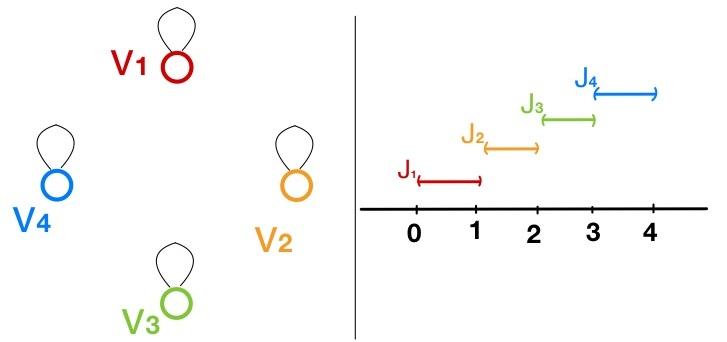
\includegraphics[width=0.6\textwidth]{recursos/capturas/201}
  \caption{A la izquierda, gráfica de intervalos de cuatro vértices sin aristas (salvo lazos), a la derecha,una representación por intervalos.}
  \label{fig:GrafInt01}
\end{figure}



    \label{exmpl:202}
    Ahora veamos si la gráfica que se muestra en \cref{fig:GrafInt01} sigue
    siendo gráfica de intervalos si a esta se le añade un arista. Para poder
    verificar esto, es necesario encontrar una nueva representación por
    intervalos. Dada la nueva incidencia, solo bastaría modificar la
    representación de los intervalos que representan a $v_1 $ y a $v_2$ es decir
    solo necesitamos que $J_1 \cap J_2 \neq \emptyset$. Así podemos simplemente
    extender el extremo derecho de $J_1$ digamos un $\varepsilon >0 $ lo
    suficientemente pequeño de tal forma que $1+\varepsilon \leq 2$, esto para
    evitar que $J_1 \cap J_3 \neq \emptyset$ pues nos generaría una adyacencia
    de $v_1 $ con $v_3$. Y respecto al resto de los intervalos $j_2, J_3, J_4$
    los conservamos iguales.    


\begin{figure}[H]
  \centering
  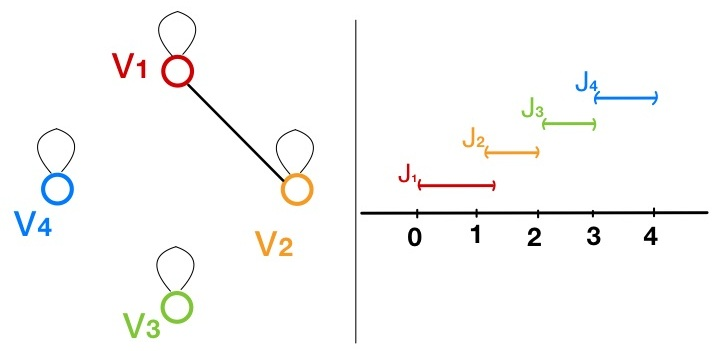
\includegraphics[width=0.6\textwidth]{recursos/capturas/202}
  \caption{A la izquierda, gráfica de intervalos de cuatro vértices con un aristas (y lazos), a la derecha,una representación por intervalos.}
  \label{fig:GrafInt02}
\end{figure}


Seguimos usando de base la gráfica de  \cref{fig:GrafInt01}, y ahora ponemos dos
adyancencias mas. Notemos que tenemos ahora un 3-camino. Y nos volvemos a
preguntar si esta nueva gráfica sigue siendo gráfica de intervalos. Y para esto
usamos una idea bastante similar a la del ejemplo pasado. Tomamos un $0 <
\varepsilon \leq 1$, y nuestros intervalos quedan como $J_i=(i-1,
i+\varepsilon)$ para $i=1,2,3$. En este punto lo único que hay que verificar es
que las adyacencias queden como se desea en la gráfica. Notemos que $J_i \cup
J_j $ si y solo si $i$ y $j$ son sucesivos. Por todo lo anterior tenemos que
esta gráfica si es de intervalos, mas aún, usando un argumento inductivo,
tenemos que cualquier k-camino es gráfica de intervalos.


\begin{figure}[H]
  \centering
  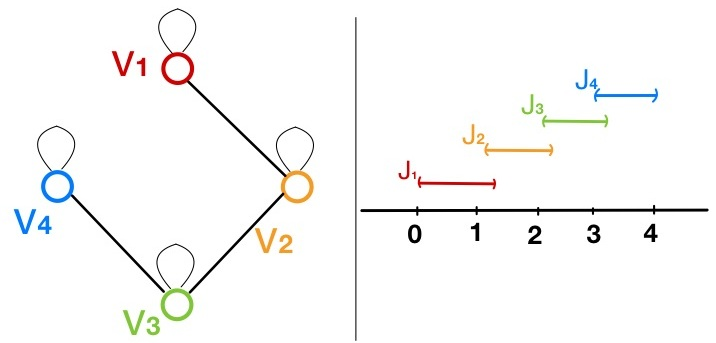
\includegraphics[width=0.6\textwidth]{recursos/capturas/203.jpg}
  \caption{A la izquierda, un 4-camino, a la derecha,una representación por intervalos.}
  \label{fig:GrafInt03}
\end{figure}

En este punto surge naturalmente la pregunta ¿Qué pasa al añadir una adyacencia
mas, es decir el 4 ciclo? ¿Es también gráfica de intervalos? Bien, intentemos
modificar la representación que dimos en \cref{fig:GrafInt03}. ¿Qué podemos
hacer? Lo único que le falta a la representación es que $J_1$ intersecte a
$J_4$. Así tenemos una primer opción, podríamos intentar extender el extremo
derecho de $J_1$ de tal forma que este rebase al tres (En la recta real). Pero
una tendremos una consecuencia inmediata, la cual es que $v_1$ es adyacente a
todos los vértices, el problema es que nos da la adyacencia de $v_1$ con $v_3$
nosotros no la buscamos, entonces descartamos esta opción.

Sin duda uno podría seguir intentando hacer modificaciones a la representación,
pero desafortunadamente nunca podremos dar con alguna que nos dé la correcta
representación del 4-ciclo, ya que en efecto el 4-ciclo no es gráfica de
intervalos.   Exploraremos algunas propiedades b\'asicas de las gr\'aficas de
intervalos en la siguiente secci\'on.

\section{Propiedades b\'asicas}

Como es de suponerse, la última afirmación de la secci\'on anterior, que resulta
ser tan contundente, debe ir respaldada por una prueba formal. A continuación
daremos una definición y un teorema, los cuales nos ayudarán a concluir que en
efecto el 4-ciclo no es de intervalos.

Decimos que una gráfica cordal es aquella en la cual todos los ciclos de cuatro
mas vértices tiene una cuerda. Esto es un arista la cual no es parte del ciclo,
pero que conecta a dos vértices dentro del ciclo.

\begin{teorema}
\label{teo:Int-Chord}
    Toda gráfica de intervalos es cordal.
\end{teorema}

\begin{proof}
    Sea G una gráfica de intervalos. Y $\{ J_v \}_{v \in V(G)}$ una
    representación de intervalos de $G$. Supongamos además que $G$ es no cordal,
    así, existe un ciclo $[v_0,v_1,v_2,...,v_{l-1},v_0]$ con $l \geq 4$, el cual
    no tiene aristas entre dos vértices no consecutivos.
    
    Notemos que $J_{v_i}$ y $J_{v_{i-1}}$ no pueden ser disjuntos, pues sus
    respectivos vértices son adyacentes al pertenecer y ser consecutivos en el
    ciclo. Por lo anterior $\forall 1 \leq i \leq n  (\exists p_i \in
    J_{v_{i-1}}\cap J_{v_i})$.
    
    Dado que por hipótesis $G$ es no cordal, $J_{i-1}$ y $J_{i+1}$ no se
    traslapan, y aunado a la tricotomía, obtenemos que $p_i$ está o bien a la
    derecha o bien a la izquierda de $p_{i+1}$. Luego, la sucesión de números
    $\{ p_i \}_{i=1}^{l-1}$ es creciente o decreciente, y justo en este punto
    surge la contradicción, pues debería suceder que $J_{l-1}$ y $J_0$ se
    intersequen, por ser la parte final del ciclo.
\end{proof}

\begin{corolario}
    Todo k-ciclo, con $k \geq 4$ no es gráfica de intervalos. 
\end{corolario}

En particular al completar el ciclo de \cref{fig:03} se tiene que ya no es
gráfica de intervalos.

Así hasta el momento hemos visto que toda gráfica de intervalos debe ser cordal.
En este punto, como dirían varios exprofesores, todo buen matemático debería
ahora preguntarse si toda gráfica cordal tiene una representación por
intervalos. Es decir veamos si el ser cordal es una condición suficiente para
ser gráficas de intervalos. Desafortunadamente, aunque al mismo tiempo
afortunadamente, para los fines literarios de esta tesis, la respuesta es no.
Veamos el siguiente ejemplo. A partir de este punto en los dibujos omitiremos
dibujar los lazos, los cuales ya sabemos que existen en toda gráfica de
intervalos.


Afirmamos que la gráfica de \cref{fig:GrafCrdlnodeInt} no es gráfica de
intervalos. Supongamos que $ \{ J_v \}_{v\in V(G)}$ es una representación de
intervalos de $G$. Así las cosas, tenemos que $I_d$ debe intersecar a $I_a$,
$I_b$ e $I_c$. Por otro lado al ser $a,b,c$ no adyacentes $I_a$, $I_b$ e $I_c$
deben ser disjuntos, de todo lo anterior se tiene que uno de estos tres
intervalos debe quedar propiamente contenido en $I_d$. Supongamos sin perdida de
generalidad que $I_a$ fue el que quedó totalmente contenido en $I_d$. Ya como
ultima nota, $I_d$ debe ser disjunto de $I_x$  ($x$ y $d$ no son adyacentes),
pero al estar $I_a$ contenido propiamente en $I_d$, no habrá forma de que $I_x$
sea disjunto con $I_d$ Por lo que no es posible que La gráfica sea de
intervalos.

\begin{figure}[H]
  \centering
  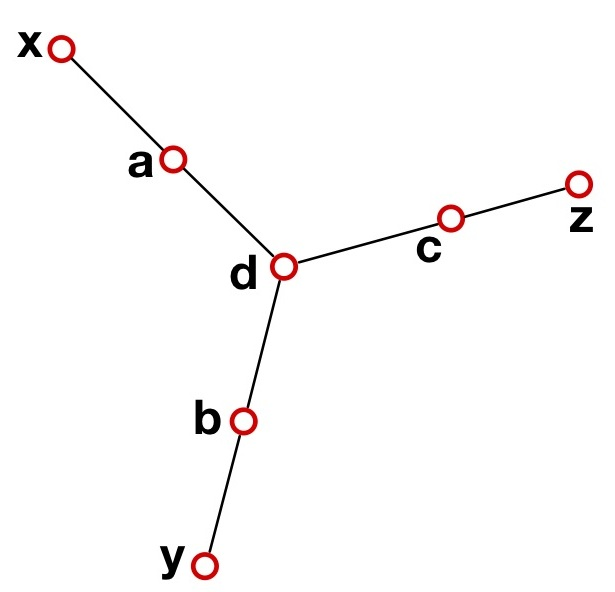
\includegraphics[width=0.3\textwidth]{recursos/capturas/204.jpg}
  \caption{Gráfica cordal la cual no es gráfica de intervalos.}
  \label{fig:GrafCrdlnodeInt}
\end{figure}

Siguiendo con el proceso del estudio de las gráficas de intervalos, ahora nos
gustaría encontrar una propiedad adicional de las gráficas de intervalos y
nuevamente preguntarnos si esta propiedad es suficiente para que la gráfica sea
de intervalos y en caso de no serlo, preguntarnos entonces si esta nueva
propiedad en junto a la propiedad de ser cordal nos den la suficiencia para ser
de intervalos. De acuerdo a lo anterior, se presentan tres actores. El primero
de ellos se presenta de forma natural al hacer un par de observaciones basadas
en la representación por intervalos de una gráfica de intervalos. Más en
especifico en observar el comportamiento de las componentes conexas de la
gráfica. Este actor veremos que resulta ser suficiente para caracterizar a las
gráficas de intervalos. Respecto a los otros dos actores, uno consiste en tener
una estructura prohibida, las tripletas asteroidales y el segundo se refiere a
una propiedad del complemento de la gráfica, el complemento debe admitir una
orientación transitiva. Cada uno de ellos se complementan con la propiedad de
ser cordal para así poder caracterizar a las gráficas de intervalos. Por el
momento veremos un par de ejemplos de gráficas de intervalos un poco mas
elaborados y veamos como surge de forma intuitiva la primer caracterización. Y
posponemos para secciones posteriores el estudio de los otros dos actores.

Una nota importante a hacer respecto a las gráficas de intervalos es pueden ser
conexas o disconexas. En \crefrange{fig:GrafInt01}{fig:GrafInt02} se exponen
gráficas de intervalos disconexas mientras que en \cref{fig:GrafInt03} se
muestra una gráfica de intervalos que es conexa. 

Como comentamos al principio del capítulo la representación por intervalos de
las gráficas ayuda a visualizar la relación de incidencia entre los vértices.
Por ejemplo, si tenemos una gráfica que es de intervalos y sucede que al unir
todos los intervalos de la representación de la gráfica esto nos da nuevamente
un intervalo, se puede concluir que la gráfica es conexa. Esta afirmación se
observa en la representación que dimos en \cref{fig:GrafInt03}, la unión de los
cuatro intervalos resulta en el intervalo $(0,4)$.

Otra propiedad importante respecto a visualizar una gráfica mediante su
representación por intervalos es que los clanes maximales son fácilmente
localizables. Mas aún dado el orden que tenemos en la recta real, los clanes
podrán ser ordenados linealmente.

Por ejemplo si uno quiere localizar los clanes maximales que contienen al
vértice $v$ nos fijamos en el intervalo $I_v$ y entonces los clanes maximales
que tienen a $v$ serán los conjuntos $C = \{w \in V(G)| I_v \cap (\bigcap I_w)
\neq \emptyset\}$. Y tales que $\nexists u \in V(G)$ tal que $I_u \cap C \neq
\emptyset$. Todo este algoritmo se simplifica de la siguiente forma, tomemos el
intervalo $I_v$, a continuación tracemos una linea vertical de tal forma que
esta interseque al máximo número posible de intervalos, entonces el clan maximal
estará conformado por aquellos vértices correspondientes a los intervalos $I_w$
tales que fueron intersecados.  

En \cref{fig:MaxClqs01} se muestra una gráfica de intervalos $G=\{ 0,1, ...,
11\}$, y su representación por intervalos se muestra en la parte inferior de la
gráfica. Denotamos sus intervalos con la misma etiqueta correspondiente al
vértice (omitiremos los puntos iniciales y finales de los intervalos pues carece
de importancia en el presente ejemplo).     
Comencemos a ver sus clanes maximales.\\
1.- Si nos fijamos en el intervalo (de etiqueta) $1$ vemos que podemos trazar
una linea vertical que intersecte al intervalo 2 (linea roja delgada), sin
embargo esta no cumple ser la linea que intersecta al mayor número de
intervalos, por ejemplo la linea roja mas gruesa no solo intersecta a los
intervalos 1 y 2 si no que también intersecta al intervalo 3. Así el primer clan
maximal que hemos detectado es $C_1$ y está conformado por los vértices
$1,2,3$.\\
2.- A continuación nos fijamos en el intervalo 2, y notamos que al trazar una
línea vertical la cual intersecte a otros intervalos las únicas posibilidades
son que la linea intersecte a los intervalos 1,2 o 2,3 o 1,2,3. Pero en
cualquiera de los tres casos, estos son clanes contenidos ya en $C_1$.\\
3.- Ahora pasamos al siguiente intervalo, notamos que en el intervalo 3, podemos
trazar la linea vertical azul, la cual intersecta a los intervalos 3, 4 y 5.
Dando pie a un nuevo clan maximal $C_2$. \\
Siguiendo este pequeño algoritmo de verificación de intersección máxima,
trazamos las lineas verticales; azul, naranja, morado, rosa y verde. Coloreamos
adicionalmente los vértices de acuerdo a los clanes a los cuales pertenecen. Así
los vértices pintados de un solo color son aquellos vértices que pertenecen a un
único clan maximal. Los vértices bicolor pertenecen a dos clanes maximales,
mientras que los tricolor pertenecen a tres clanes maximales. Con todo lo
anterior los clanes maximales de $G$ son $C_1, C_2, ..., C_6$ estos están
coloreados del color correspondiente a la linea vertical.    


\begin{figure}[H]
  \centering
  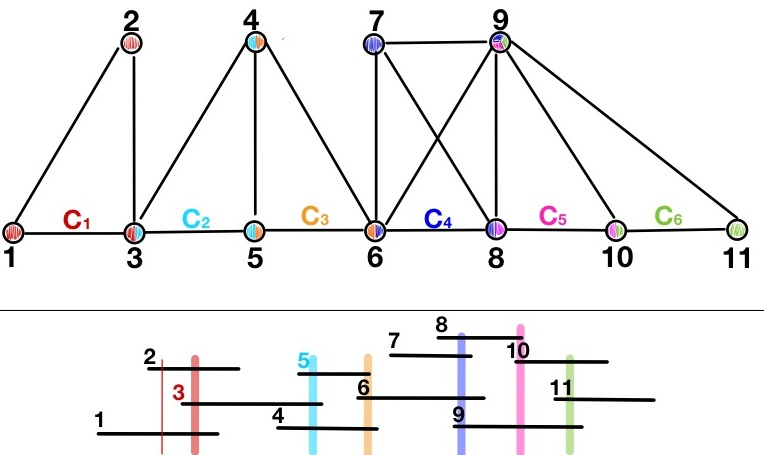
\includegraphics[width=0.8\textwidth]{recursos/capturas/208.jpg}
  \caption{Localización de clanes maximales dada la representación por intervalos de una gráfica.}
  \label{fig:MaxClqs01}
\end{figure}

\Cref{fig:MaxClqs02} es un ejemplo mas en cual mostramos la ventaja de contar
con la representación por intervalos de una gráfica. El proceso de colocar
lineas verticales sirve para identificar rápidamente los clanes maximales
$C_1,C_2, C_3, C_4, C_5, C_6, C_7, C_8$.

En \cref{sec:SbGrfcs} se introdujo el concepto de vértice simplicial. Notemos
que también al contar con la representación por intervalos de una gráfica, nos
facilita la tarea de reconocerlos, pues los vértices simpliciales serán aquellos
vértices para los cuales sus intervalos  correspondientes solo son intersectados
por una linea vertical correspondiente a clanes maximales. En
\cref{fig:MaxClqs02}, al fijarnos en la representación por intervalos, vemos que
los intervalos 1,2,3,4 solo son intersectados por una linea correspondiente a un
clan maximal, mientras que el intervalo 5, es intersectado por dos, la naranja y
la azul. Así en el ejemplo en cuestión tenemos que los vértices simpliciales son
los monocrom\'aticos, es decir $1,2,3,4,9,14,15,16$ todos ellos son vértices
simpliciales.

\begin{figure}[H]
  \centering
  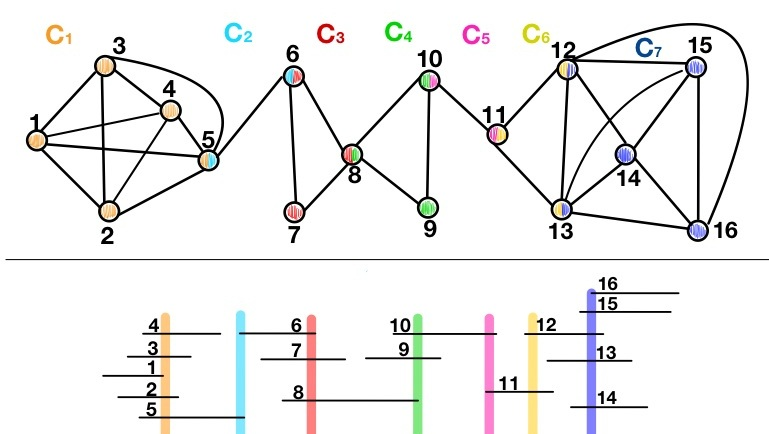
\includegraphics[width=0.8\textwidth]{recursos/capturas/209.jpg}
  \caption{Localización de clanes maximales dada la representación por intervalos de una gráfica.}
  \label{fig:MaxClqs02}
\end{figure}

Una vez que uno cuenta con un la representación por intervalos de una gráfica,
la representación sugiere un ordenamiento muy natural de los clanes maximales,
de izquierda a derecha. Por ejemplo en \cref{fig:MaxClqs02} podemos ordenar los
clanes maximales como $(C_1,C_2, C_3, C_4, C_5, C_6, C_7)$. Alternamente si
proponemos la representación por intervalos que resulta de reflejar, por una
linea vertical a la izquierda del intervalo 16, la representación dada en
\cref{fig:MaxClqs02}. Ahora se obtiene el ordenamiento
$(C_7,C_6,C_5,C_4,C_3,C_2,C_1)$. Ciertamente uno puede dar cualquier
ordenamiento de los clanes maximales de la gráfica, sin embargo los que surgen
de forma natural dada la representación por intervalos, tienen una peculiaridad.
Los clanes que tienen a un vértice $v$ aparecen consecutivamente en el orden
dado. Veamos esto. Supongamos que $G$ es una gráfica de intervalos y que
$\{C_i\}_{i=1} ^n$ es el ordenamiento de sus clanes maximales dado por la
representación de intervalos, supongamos adicionalmente que $v\in C_k$ y $v\in
C_l$ y $k<j<l$ entonces $v\in C_j$. Esto se puede observar en
\crefrange{fig:MaxClqs01}{fig:MaxClqs02}. 



    \begin{comment}
    Sin embargo ambos ordenes son dependientes de la representación por
    intervalos que uno haya elegido. En \cref{fig:OrdMaxClns} tenemos una
    estrella de 5 picos y a la derecha se muestran tres posibles
    representaciones por intervalos de dicha gráfica. La estrella tiene como
    clanes maximales a los conjuntos $C_{i-1}=\{1,i\}$ con $i \in
    \{2,3,4,5,6\}$, es decir un pico de la estrella acompañado del centro. En la
    representación por intervalos de la parte superior se ocurre inmediatamente
    dos ordenaciones de los clanes maximales, $(C_1,C_2,C_3,C_4,C_5)$ y
    $(C_5,C_4,C_3,C_2,C_1)$. De forma análoga las representaciones del centro y
    de la parte inferior nos sugieren cada una dos ordenaciones, de derecha a
    izquierda y de izquierda a derecha. En general, en este acaso particular
    cualquier permutación de los clanes nos da una ordenación. 
    
    \begin{figure}[H]
      \centering
      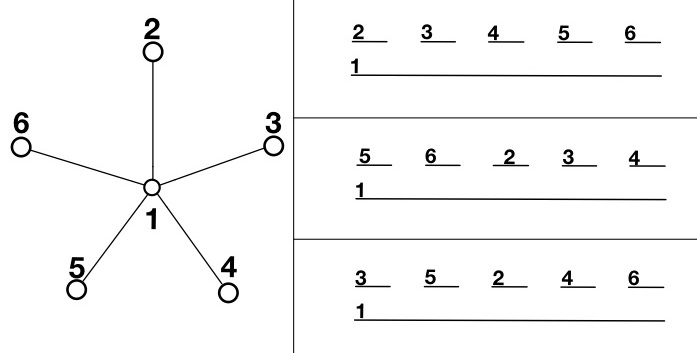
\includegraphics[width=0.7\textwidth]{recursos/capturas/OrdMaxClns.jpg}
      \caption{Ordenamientos de los clanes maximales de la estrella.}
      \label{fig:OrdMaxClns}
    \end{figure}
    
    La finalidad de todo lo anterior es para hacer notar que, si bien los clanes
    pueden ser ordenados, necesitamos una característica la cual no dependa de
    la representación, si no mas bien de la interacción entre los vértices y los
    clanes maximales. Así notemos de \crefrange{fig:208} cualquier orden que
    demos de 
\end{comment}

En efecto, la propiedad de poder ordenar los clanes maximales de tal forma que
para todo vértice $v\in V$ los clanes maximales que contienen a $v$ aparecen
consecutivamente en el orden, es una condición necesaria y suficiente para ser
una gráfica de intervalos. A este tipo de ordenamiento de los clanes tambi\'en se les suele decir la descomposici\'on consecutiva de $G$ en gr\'aficas primas que consta de clanes. 

A continuaci\'on formalizamos las ideas anteriores, pues resultan \'utiles para resultados posteriores. 

Dada una gr\'afica $G$, decimos que $G_0,G_1,\dots,G_n$ es una descomposici\'on de $G$ en gr\'aficas primas, si sucede que $G=G_0 \cup G_1\cup \cdots \cup G_n$ donde cada $G_i$ es una gr\'afica prima, es decir $G_i$ no tiene clanes separadores para todo $0\leq i \leq n$. Adem\'as se debe cumplir que $S_i=(G_0\cup G_1\cup \cdots \cup G_{i-1})\cap G_i$ es un clan el cual est\'a propiamente contenido en $G_i$ y en $G_0\cup G_1\cup G_{i-1}$ tales conjuntos $S_i$ son llamados clanes de adjunci\'on de la descomposici\'on en gr\'aficas primas en cuesti\'on. 

Veamos un par de ejemplos sencillos sobre la descomposición de gráficas en gráficas primas. Como primer ejemplo, tenemos la gráfica $G$ que consta de tres vértices y una sola arista, digamos $V(G)=\{v_0,v_1,v_2\}, E(G)=\{v_1,v_0\}$. Dicha gráfica la podemos descomponer de la siguiente manera $G_0,G_1$ con  $V(G_0)=\{v_0,v_1\}, E(G_0)=\{ \{v_0,v_1\} \} $ y con $V(G_1)=\{v_2\}, E(G_1)=\emptyset $. En este caso, es claro que tanto $G_0$ como $G_1$ ambas carecen de clanes separadores, y por tanto son gráficas primas, en segundo lugar $G_0\cap G_1= \emptyset$ la cual es por vacuidad una gráfica completa. En este mismo ejemplo, nos podemos percatar que se pudo tomar otra descomposición en gráficas primas, simplemente intercambiando los nombres de las gráficas primas, es decir renombrarlas, que $G_0$ sea ahora la gráfica $G_1$ y que $G_1$ sea ahora $G_0$. 

Como segundo ejemplo, tenemos un cuatro ciclo $(v_0,v_1,v_2,v_3)$, en este caso el mismo cuatro ciclo es ya una gráfica prima, no tiene clanes separadores. Los únicos conjuntos de corte, son pares de vértices opuestos, pero estos no conforman un clan. Así, en este caso, la descomposición es el mismo cuatro-ciclo. Un tercer ejemplo, lo podemos construir a partir del cuatro-ciclo, añadiendo una arista diagonal, supongamos $\{v_0,v_2\}$, con esta pequeña modificación, ahora la gráfica ya no es prima, ya que ahora el conjunto $\{v_0,v_2\}$ es un conjunto de corte, más aún es un clan de corte. Dada esta situación, procederemos a buscar otra descomposición en gráficas primas, proponemos $G_0,G_1$ como $G_0=(\{v_0,v_1,v_2 \},\ \{ \{v_0,v_1\},\{v_1,v_2\},\{v_2,v_0\} \} )$ y $G_1= ( \{v_0,v_3,v_2\}, \ \{ \{v_0,v_3\},\{v_3,v_2\},\{v_2,v_3\} \} )$. Así definidas las gráficas, es fácil verificar que ambas son gráficas primas, ya que son gráficas completas y entonces no tienen clanes de corte, además $G_0\cap G_1 = \{v_0,v_2 \}$ y este es un clan. Por lo tanto, $G_0, G_1$ es una descomposición en gráficas primas.
Un ejemplo más es el seis-ciclo, $(v_0,v_1,v_2,v_3,v_4,v_5)$, con un vértice extra $v_6$ y las siguientes adyacencias adicionales $\{v_6,v_0\},\{v_6,v_2\},\{v_6,v_4\}$. En la figura 6464646, se ilustra dicha gráfica, y las gráficas primas de descomposición son las siguientes $G_0=\{v_0,v_1,v_2,v_6\},G_1= \{v_2,v_3,v_4,v_6\},G_2=\{v_4,v_5,v_0,v_6\}$ (las gráficas inducidas).

Con esté último ejemplo, mostramos que las gráficas primas en una descomposición, no son necesariamente clanes, sin embargo hay casos en los que precisamente las gráficas primas de descomposición son clanes, cuando este sea el caso, diremos que tenemos una descomposición en gráficas primas que consta de clanes, o simplemente una descomposición en clanes, puesto que cada clan es de por sí una gráfica prima.

Por supuesto, también tenemos el ejemplo de \cref{fig:MaxClqs02}. La gr\'afica $G$ se puede descomponer en los siete clanes maximales exhibidos, los cuales son claramente gráficas primas, así $G=C_1 \cup \dots \cup C_7$ y los respectivos clanes de adjunci\'on en este caso son aquellos v\'ertices multicolor. Algo aún más interesante de nuestro ejemplo es el hecho de que los clanes cumplen lo siguiente, para cada $1\leq i\leq n$ se tiene que $S_i\subseteq C_{i-q}$. Esto no pasa en general, pero en el caso de las gr\'aficas que son de intervalos tenemos esta interesante propiedad. Así si $G$ es una gráfica y $G_0,G_1,\dots,G_k$ es una descomposición de $G$ en gráficas primas decimos que la descomposición es consecutiva si y solo si $v\in G_i, v\in G_h$ con $i<j<h$ implica que $x\in G_j$. Además si cada $G_i $ es un clan, decimos que tenemos una descomposici\'on consecutiva de $G$ en clanes.

Veamos propiedades interesantes referentes a las descomposiciones en gráficas primas. La primer observación que haremos es que dada una gráfica $G$ y una descomposición en gráficas primas $G_0,G_1,\dots,G_{k}$ de $G$, los clan de adjunción $S_i$ separan a $G$, mas precisamente, los vértices de $(G_0\cup \cdots \cup G_{i-1})- S_i$ están separados de los vértices de $G_i- S_i$. En efecto esto sucede, ya que todas las aristas que hay después de quitar el clan $S_i$ son aristas $uv$ con $u,v\in G_0\cup G_1 \cup \cdot \cup G_{i-1}$ o bien con ambos vértices en $G_i$, es decir no hay aristas conformadas por vértices en componentes distintas. Así queda claro que en efecto $S_i$ separa a $G$. Una gráfica es cordal si y solo si esta  tiene una descomposición en clanes. Veamos mediante un argumento inductivo sobre el número de vértices de $G$ que $G$ se puede descomponer en unión de clanes. Claramente si $|G|$ es uno, entonces $G$ es un clan y entonces se representa como unión de clanes. Ahora, supongamos que si el cardinal de $G$ es menor que $k$ entonces $G$ se puede descomponer como unión de clanes. Finalmente si $G$ tiene orden $k+1$ y además no es un clan, entonces por el teorema 1.5.3 sabemos que $G$ tiene un vértice simplicial, digamos $v$, así, consideremos $K$ como la subgráfica completa inducida por $v$ y todos sus vecinos. Tomemos ahora, $G'=G-K$, por hipótesis inductiva, hay una descomposición en clanes de $G'$, digamos $K_1,K_2\dots, K_l$. Finalmente podemos concluir que $K_1,K_2\dots, K_l, K$ es una descomposición de $G$ en clanes. Además notemos que el teorema 1.5.4 nos lleva a concluir que los conjuntos $S_i$ son efecto clanes. Ahora, supongamos que tenemos una gráfica $G$ la cual podemos descomponer en clanes, y sea $(u_1,u_2,u_3,u_4,u_1)$ un cuatro ciclo, veamos que forzosamente debe haber una cuerda. Como $G$ tiene una descomposición en gráficas primas, debe suceder que cada $u_i$ pertenece a $G_j$ algún clan. Como $u_1$ es adyacente a $u_2$ y a $u_4$, entonces ambos $u_2, u_4$ pertenecen a $G_j$ es decir luego, debe haber un arista entre $u_2$ y $u_4$. Por lo que $G$ es una gráfica cordal.

Supongamos que $G_0,G_1,\dots,G_k$ es una descomposición consecutiva de $G$ en clanes. Entonces también tenemos las siguientes propiedades. $G_k,\dots,G_1,G_0$ es también una descomposición consecutiva de $G$ en clanes. Verificar este resultado es inmediato, pues, cada subgráfica $G_i$ es completa por hipótesis, así como cada $S_i$, y además se mantiene que si $i>j>h$ y $v\in G_i$ y $v\in G_h$ entonces $v\in G_j$. Nuestra segunda propiedad nos dice que para todo índice $i$ entre 1 y $k$, tenemos que $(G_0\cup \cdots \cup G_{i-1})-S_i$ está separado de $(G_i \cup \cdots \cup G_k)-S_i$. Veamos esto por inducción, sobre el número de componentes en la descomposición. Si tenemos una única componente el resultado no es relevante, cuando tenemos dos componentes el argumento que prueba nuestra proposición es que las aristas están compuestas únicamente por vértices de la misma componente. Así supongamos que cualquier gráfica la cual tiene una descomposición consecutiva en $k$ clanes, cumple nuestra proposición. Ahora supongamos que tenemos una gráfica $G$ y que esta tiene una descomposición consecutiva en $k+1$ clanes. Veamos algunos casos que surgen en este punto. Si $i\in \{1,k\}$ entonces nuevamente es sencillo ver que separa por la naturaleza de las aristas. Ahora supongamos que $i\notin \{1,k\}$, veamos que dado $u\in (G_0\cup \cdots \cup G_{i-1})-S_i $ y $v \in (G_i \cup \cdots \cup G_k)-S_i $ estos quedan separados. Caso 1, sea $i_u$ el índice correspondiente al clan en el cual se encuentra $u$ y sea $j_v$ el índice del clan en el cual se encuentra $v$. Ahora, si $j_v-i_u\leq k$ entonces podemos suponer que $G_l$ con $l\in \{0,k+1\}$ es tal que no contiene a $u$ ni a $v$. Así podemos considerar la gráfica $G^*=G-G_l$ y entonces por hipótesis inductiva en $G^* - S_i$ los vértices $u,v$ están separados. Luego, al considerar nuevamente la gráfica $G$, $u,v$ vuelven a quedar separados. Ahora el caso de mayor interés es cuando $j_v-i_u = k+1$, en este caso $u\in G_0$ y $v_\in G_{k+1}$. Ahora tomemos un $uv$-camino, digamos $(u,x_1,\dots,x_n,v)$, luego, tomamos $x_j$ donde $j =\min\{i | x_i \in G_{k}, v_\notin C_{k+1}\}$, este debe existir, ya que si no, esto implicaría que todo el $uv$-camino pertenece a $G_{k+1} $. Así las cosas, por hipótesis inductiva, debe suceder que $u$ y $x_j$ están separados en $G-S_i$, luego $u,v$ quedan separados en $G$.

Ahora supongamos que $T\subseteq V(G)$ el cual separa a $G$, veamos que entonces $T$ contiene a algún $S_i$. Como $T$ es separador, consideremos algún subconjuto de $T$ que sea separador mínimo. Ya vimos que si una gráfica tiene una descomposición consecutiva en clanes, entonces $G$ es una gráfica de intervalos, en particular una gráfica cordal, entonces tenemos que cualquier conjunto separador mínimo es un clan. Es decir $T$ en efecto contine a un clan separador. Otra observación sencilla es que $G_i $ con $i\in \{1,\dots, k-1\}$ separa a $G$, esto es directo del hecho de tener una descomposición consecutiva, pues $S_{i-1}\subseteq G_i$ y ya vimos que los clanes de adjunción en efecto separan a $G$. Por otro lado, si $G_i$ no separa a $G$, entonces $i\in \{0,k\}$. 
El último resultado referente a las descomposiciones cosecutivas en clanes maximales, es que para cualquier subgráfica $H$ de $G$ nosotros obtenemos una descomposición consecutiva de $H$ en clanes maximales al intersecar cada clan $G_i$ con $H$, así la descomposición es $H\cap G_0, H\cap G_1, \dots, H\cap G_k$, para verificar que esta es en efecto una descomposición consecutiva en clanes, hay que verificar que cada $G_i\cap H$, es en efecto un clan, lo cual ciertamente se cumple pues $G_i\cap H$ es un clan al ser una subgráfica de un clan. Luego cada $S_i\cap H$ por la misma razón vuelve a ser un clan. Finalmente basta ver que $S_i\cap H \subseteq G_{i-1} \cap H$ pero nuevamente esto vuelve a ser inmediato del hecho que $S_i$ es subconjunto de $G_{i-1}$. 

De momento dejaremos estos resultados y posteriormente los retomaremos para probar que el tener una descomposición consecutiva en clanes maximales es una condición suficiente para garantizar que 


\section{Orientaciones transitivas}
Como vimos en el capitulo anterior, que una gráfica sea cordal no es una
condición suficiente para que una gráfica sea de intervalos. En esta sección
introducimos una propiedad adicional, la cual nos da la suficiencia.

Dada un gráfica $G$, una \indice{orientación transitiva} consiste en, nosotros
poder asignar una orientación a las aristas de la gráfica formando así una
gráfica dirigida $(V(G),F)$ de tal forma que $ab\in F$ y $bc\in F$ implica que
$ac\in F$ $\forall a,b,c \in V(G)$

Veamos el siguiente ejemplo bastante sencillo.

Tenemos un 3-ciclo. Y nos preguntamos si este tiene la propiedad de orientación
transitiva. Para esto debemos asignar dirección $F$ a sus aristas, de tal forma
que $ab\in F$ y $bc\in F$ implica que $ac\in F$. Por ejemplo, damos la
orientación $F_1$ tal que; al arista diagonal de la izquierda le damos sentido
de arriba hacia abajo, al arista horizontal le damos sentido de izquierda a
derecha, y finalmente al arista diagonal restante (de la derecha) debe ir de
arriba hacia abajo.
    
Como un segundo ejemplo damos la orientación $F_2$ tal que; al arista diagonal
de la izquierda le damos sentido de abajo hacia arriba, al arista horizontal le
damos sentido de derecha a izquierda, y al arista diagonal de la derecha abajo
hacia arriba.

Es fácil comprobar que este par de orientaciones son en efecto un par de
orientaciones transitivas de la gráfica $G$.


\begin{figure}[H]
  \centering
  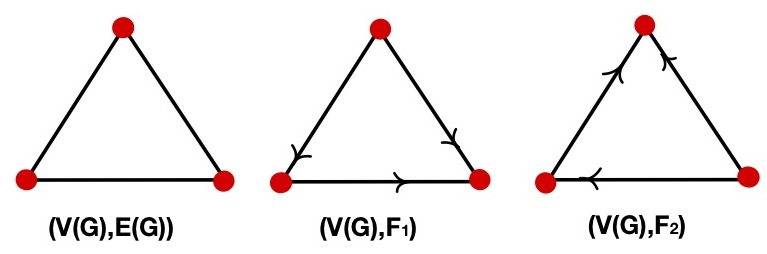
\includegraphics[width=0.6\textwidth]{recursos/capturas/205.jpg}
  \caption{ Gráfica $G$ y un par de orientaciones transitivas $F_1$ y $F_2$ .}
  \label{fig:GrfTrnsOrtbl}
\end{figure}

Aquellas gráficas no dirigidas que pueden ser transitivamente orientables, les
llamaremos \textbf{gráficas} \indiceSub{gráfica}{de comparabilidad}.

A continuación dejamos un par mas de gráficas de comparabilidad y sus
respectivas orientaciones $H$ y $E$.

\begin{figure}[H]
  \centering
  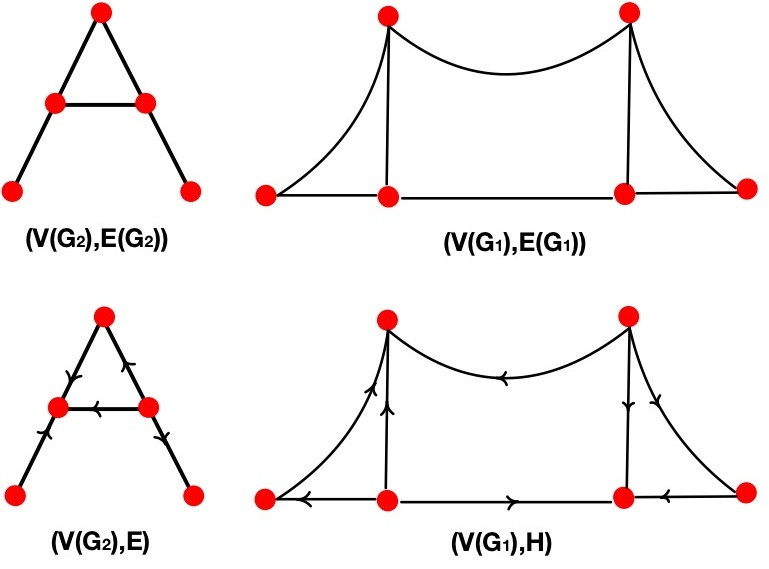
\includegraphics[width=0.6 \textwidth]{recursos/capturas/206.jpg}
  \caption{Gráficas $G_1$ y $G_2$ y las orientaciones transitivas $H$ y $E$ de $G_1$ y $G_2$ respectivamente.}
  \label{fig:206}
\end{figure}

Para terminar de nutrir el concepto de gráfica de comparabilidad, veamos un
ejemplo de una gráfica la cual no es transitivamente orientable.

En el siguiente ejemplo tenemos el 5-ciclo, y afirmamos que no es posible dar
una orientación de las aristas de tal forma que esta resulte una orientación
transitiva.
    
Veamos la \cref{fig:207}. Tratemos de dar una orientación transitiva, empecemos
tomando un vértice cualquiera, por ejemplo tomamos el vértice $A$ y tomamos una
de sus aristas y le asignamos un sentido a esta, por ejemplo como se ve en la
gráfica de en medio, asiganamos una flecha que va de $A$ a $B$. Continuemos con
$B$ podemos ahora asignarle a su arista restante la dirección hacia $C$. Sin
embargo, con esta orientación tendríamos que debería haber una flecha de $A$ a
$C$ (Ya que queremos que la orientación sea transitiva), lo cual no puede ser.
Esto nos dice que el arista de $BC$ debe ser orientada de $C$ a $B$, como la
ilustración de la derecha indica.
    
En general debemos de evitar que haya 2-caminos cuyas  flechas tengan la misma
orientación (Gráfica del centro). Así siguiendo la asignación de orientaciones,
el arista $CD$, debe ir de $C$ hasta $D$, continuando, el arista $DE$ debe ir de
$E$ a $D$ y siguiendo de esta forma, el arista $EA$ debería ir de ... ¿$E$ a
$A$? ¿$A$ hacia $E$? ¡Ambos casos nos llevan a flechas con las que no contamos!
Aquí se observa la imposibilidad de encontrar una orientación transitiva para
$C_5$

Y es fácil observar, que este fenómeno puede ser fácilmente extendible hacia los
ciclos de longitud $k$ impar, $k\geq 5$

\begin{figure}[H]
  \centering
  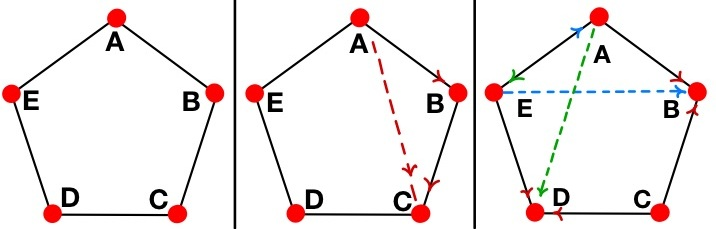
\includegraphics[width=0.7\textwidth]{recursos/capturas/207.jpg}
  \caption{$C_5$ no es gráfica de comparabilidad.}
  \label{fig:207}
\end{figure}

Una vez ya asimilado el concepto, regresamos a nuestra tarea, queríamos ver si
esta es una propiedad que nos ayude a caracterizar a las gráficas de intervalos.
La respuesta, como es de esperarse, es que si nos ayudará a caracterizar a las
gráficas de intervalos. Algo interesante que veremos y probaremos a continuación
es que el complemento de una gráfica de intervalos es gráfica de comparación.

\begin{teorema}
    \label{teo:Int-Comprbldd}
    El complemento de una gráfica de intervalos es una gráfica de comparación.
\end{teorema}

\begin{proof}
    Sea $G=(V,E)$ una gráfica de intervalos y sea $\{I_v \}_{v\in V(G)}$ una
    representación de intervalos de $G$. Y ahora consideremos $ \bar{G} =(V,
    \bar{E})$ aquí buscamos encontrar un orientación $F$ de las aristas de
    $\bar{E}$ la cual sea transitiva.
    
    La definimos de la siguiente forma.
    
    $xy\in F \iff I_x<I_y$ $(\forall xy\in \bar{E})$ Donde entendemos que $I_x$
    esta a la izquierda de $I_y$ si, $\forall a\in I_x, \forall b \in I_y(a<b)$

    Finalmente esta orientación resulta ser transitiva como mera consecuencia de
    la transitividad de $\mathbb{R}$. $(I_x < I_y) \wedge (I_y < I_z)
    \Rightarrow (I_x<I_z) $
\end{proof}

Ya hemos advertido que nuestra caracterización de las gráficas de intervalos,
necesita de la propiedad cordal y que el complemento sea una gráfica de
comparación. Sin embargo, es necesario comprobar antes si no es suficiente el
hecho de que una gráfica satisfaga que su complemento es de comparabilidad, para
garantizar que la gráfica es de intervalos. Un ejemplo muy sencillo para exhibir
la insuficiencia es el 4-ciclo sin cuerdas. Es decir tomamos a $G=C_4$, luego
$\bar{G}$ consta de solo dos aristas y se cumple que es orientable
transitivamente casi por vacuidad.

Por lo tanto, se hace visible la necesidad de una segunda propiedad. En el
siguiente teorema damos la caracterización completa.

\begin{teorema}
\label{teo:Crctzn1}
    $G$ es gráfica de intervalos si y solo si $G$ es cordal y su complemento es
    gráfica de comparabilidad.
\end{teorema}

\section{Tripletas asteroidales}
\label{sec:AstTrpls}
Por ultimo introducimos una estructura la cual es imposible tener en una gráfica
la cual es de intervalos, y este hecho complementa la propiedad cordal para
caracterizar a las gráficas de intervalos.

Dada una gráfica $G$. Decimos que tres vértices distintos $a_1,a_2,a_3$ forman
una \indice{tripleta asteroidal} si y solo si cualesquiera de ellos dos son
conectados por un camino el cual evita al tercer vértice y todos sus vecinos.
Una gráfica la cual tenga una tripleta asteroidal es llamada
\indiceSub{gráfica}{asteroidal}. En \cref{fig:GrafAstrdl} exhibimos una gráfica
la cual tiene una tripleta asteroidal. Más en especifico, los vértices $1,5,10$
conforman una tripeta asteroidal, ya que por ejemplo podemos tomar $(1,2,4,7,5)$
la cual es una 1,5-trayectoria y esta evita a la vecindad cerrada del vértice
10, también se tiene que $(1,2,4,8,10)$ es una 1,10-trayectoria que evita a
$V[10]$, la vecindad cerrada del vértice 10 y finalmente se tiene la trayectoria
$(5,7,4,8,10)$ la cual es una 5,10-trayectoria que evita a $V[1]$.

\begin{figure}[H]
  \centering
  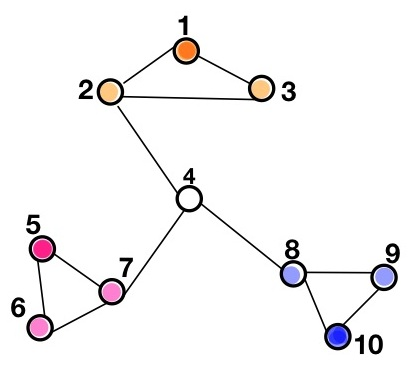
\includegraphics[width=0.5\textwidth]{recursos/capturas/Ast-Trpl.jpg}
  \caption{Gráfica asteroidal}
  \label{fig:GrafAstrdl}
\end{figure}

A continuación mostramos que es incompatible el hecho de que una gráfica tenga
una enumeración consecutiva de sus clanes maximales y la presencia de tripletas
asteroidales. Sea $G$ una gráfica de intervalos y $x,y,z \in V(G)$ una terna
arbitraria de vértices de $G$. Supongamos adicionalmente que $\{C_i\}_{i=1}^n$
es una enumeración consecutiva de los clanes maximales de $G$. Supongamos sin
pérdida de generalidad que $x\in C_i, y \in C_j, z\in C_h$ e $i\leq j \leq h$.
Luego cualquier $xz$-camino debe pasar por $C_j$, esto es no puede evitar a $y$
o algún vecino de $y$. Por ende no puede haber tripletas asteroidales en una
gráfica que tenga una enumeración consecutiva de clanes maximales. Luego,
asumiendo verdadero \cref{teo:Int-MaxClns}, se deduce que es imposible la
presencia de tripletas asteroidales en una gráfica de intervalos. Este hecho se
ve reflejado en el teorema de Lekkerkerker y Boland, que enunciamos a
continuación.

\begin{teorema}
    \label{teo:Int-Ast-free}
    Una gráfica finita $G$ es de intervalos si y solo si es cordal y no tiene
    tripletas asteroidales.
\end{teorema}

Con todo lo anterior, podemos dar paso al siguiente teorema que caracteriza a
las gráficas de intervalos.

\begin{teorema}
\label{teo:CarGrfsInt}
    Sea $G $ una gráfica. Las siguientes proposiciones son equivalentes.\\
    i) $G$ es gráfica de intervalos.\\
    ii) $G$ es cordal y su complemento es gráfica de comparabilidad.\\
    iii) $G$ tiene una enumeración consecutiva de sus clanes maximales.\\
    iv) $G$ es cordal y no tiene tripletas asteroidales. 
\end{teorema}

\begin{proof}
    i)$\to$ ii) En \cref{teo:Int-Chord} y \cref{teo:Int-Comprbldd} probamos que
    el hecho de ser gráfica de intervaos implica que la gráfica debe ser cordal
    y su complemento es necesariamente de comparabilidad, por lo que esta primer
    implicación queda cubierta.
    
    ii) $\to$ iii) Supongamos que $(G,E)$ es una gráfica cordal y que $(\bar{G},
    \bar{E})$ es gráfica de comparación, con $F$ un ordenamiento transitivo de
    $\bar{E}$. A continuación damos un ordenamiento, el cual afirmamos que
    ordenamiento lineal de $\Sigma$ el conjunto de todos los clanes maximales de
    $G$. Dados  $A_1, A_2$ clanes maximales, definimos la relación $<$ como $A_1
    < A_2$ si y solo si hay una flecha de la orientación transitiva $F$, desde
    $A_1$ hasta $A_2$, es decir que existan vértices $a_1 \in A_1$ y $a_2 \in
    A_2$ tales que $(a_1,a_2)\in F$. Ahora deberemos comprobar que dicha
    relación está bien definida, por lo que hay que garantizar dos cosas. En
    principio que dados dos clanes maximales, en efecto exista una flecha de $F$
    que los conecte. Como segunda punto habrá que verificar que en caso de
    existir un par de flechas en $F$, que unan a $A_1$ y $A_2$ estas tengan la
    misma orientación. Para probar lo primero, tomemos $A_1,A_2$ un par de
    clanes maximales de $G$ ahora supongamos que no existe ninguna flecha en $F$
    que este conformada por un vértice en $A_1$ y otro en $A_2$. Esto nos
    llevaría por definición de complemento que para todo par de vértices $a_1\in
    A_1$ y $a_2 \in A_2$,  $a_1a_2\in E$ o $a_2a_1\in E$, lo que nos lleva a que
    $A_1 \cup A_2$ es una clan de $G$, lo que contradice la maximalidad tanto de
    $A_1$ como de $A_2$. Ahora veamos vía contradicción que el segundo punto es
    satisfecho. Supongamos que tenemos un par de flechas que están conformadas
    por elementos de $A_1$ y $A_2$ pero que tienen sentidos contrarios, es decir
    tomamos $(a,b)\in F$ y $(d,c)\in F$ con $a,c \in A_1$ y $b,d\in A_2$,
    notemos que si $a=c $ o $b=d$ por transitividad se llega a una
    contradicción, en el primer caso $a=c$ se tiene que $(a,b), (d,a)\in F$
    luego $(a,a)\in F$ pero al ser $G$ reflexiva esto no puede ser. El segundo
    caso es totalmente análogo. Ahora veamos que al asumir que los cuatro
    vértices son distintos entre sí, sigue arrojándonos una contradicción. En
    este caso, tenemos que $ac, bd\in E$ al pertenecer a los mismos clanes
    maximales, adicionalmente tenemos que $ad$ y $bc$ no pueden ser ambas
    aristas de $E$ pues de serlo tendríamos el 4-ciclo $(a,d,b,c,a)$ y al ser
    $G$ cordal se llegaría a $ab\in E$ o $cd\in E$ lo que no es posible al
    pertenecer ambos a $\bar{E}$. Luego podemos asumir sin perdida de
    generalidad que $ad \in \bar{E}$. Si se tiene que $(a,d)\in F$ usando la
    transitividad y que $(d,c)\in F$ se llega a que $(a,c)\in F$ y en particular
    $ac\in \bar{E}$ lo que es imposible ya que $a$ y $c$ pertenecen al mismo
    clan. De forma análoga, si $(d,a)\in F$ usando transitividad, se tiene que
    $(d,b)\in F$ y nuevamente se llega a una contradicción al pertenecer ambos
    al mismo clan. Por todo lo anterior, dados dos clanes maximales, y dos
    flechas incidentes en estos, las flechas tienen la misma orientación.
    Finalmente verifiquemos que en efecto es un ordenamiento lineal de $\Sigma$.
    Ya hemos visto que cualesquiera dos clanes maximales, estos siempre tienen
    una flecha que los une, así cualesquiera dos clanes siempre son comparables.
    Ahora veamos que se tiene la transitividad, supongamos que $C_1,C_2, C_3$
    son tres clanes maximales de $G$ tales que $C_1<C_2$ y $C_2 <C_3$, por como
    esta definida la relación, existen $w\in C_1, x,y\in C_2, z\in C_3$ de tal
    forma que $wx, yz \in F$ luego si $xz \in \bar{E}$ o $wy \in \bar{E}$ usando
    el hecho que las flechas tienen la misma orientación, y la hipótesis de que
    la orientación es transitiva, se llega a que $wz \in F$ y así $C_1 < C_3$.
    Así podemos suponer que $wy, xz \in E$, esto aunado al hecho de que $x,y\in
    C_2$ y $C_2$ es clan, se tiene que $wz\notin E$ ya que en caso contrario se
    tendría que hay un 4 ciclo sin cuerdas $(w,y,x,z,w)$, lo que por hipótesis
    no es posible al suponer $G$ cordal. Así $wz\in \bar{E}$ y mas aún $wz \in
    F$ ya que si $zw\in F$ al ser $F$ orientable transitivamente $zx \in F$ lo
    que no es posible pues $yz\in F$ y se tendrían un par de flechas incidentes
    de $C_2, C_3$ en sentidos opuestos. Por lo que, la relación es transitiva.
    Finalmente supongamos que $\Sigma$ ha sido ordenado y que ${C_i}_{i=1}^m$ es
    el ordenamiento de los clanes con $C_i<C_j si i<j$ veamos que si
    $C_i<C_j<C_k$ y $x\in C_i $, $x\in C_k$ entonces $x\in C_j$. Veamos vía
    contradicción que esto sucede. Supongamos entonces que $x\notin C_j$.
    Tomemos a continuación $y\in C_j$ tal que $xy\notin E$ esto nos lleva a que
    $xy\in bar{E}$ y aunado a $C_i<C_j$ se tiene que $xy\in F$ por otro lado
    $C_j< C_k$ nos lleva a que $yx\in F$ lo que nos es posible. Por lo tanto
    acabamos de exhibir una enumeración consecutiva de los clanes maximales de
    $G$.

    iii) $\to$ i) Supongamos que hay una enumeración consecutiva de los clanes
    maximales de $G$, ahora para cada vértice $x$ definimos $I(x)$ como el
    conjunto de todos los clanes maximales que tienen a $x$. Los conjuntos
    $I(x)$ así definidos son intervalos en el conjunto linealmente ordenado
    $(\Sigma,<)$. Ahora hay que probar que $xy\in E \Leftrightarrow I(x)\cap
    I(y)\neq \emptyset$. Si $xy\in E$ entonces debe existir un clan maximal $C$
    tal que $x,y \in C$ luego $C\in I(x)$ y $C\in I(y)$. Así $I(x)\cap I(y)\neq
    \emptyset$, ahora si $I(x)\cap I(y)\neq \emptyset$ entonces existe $C\in
    I(x)\cap I(y)$ y así $x,y\in C$. Luego al pertenecer al mismo clan, se tiene
    que $xy\in E$. Por lo que $G$ es de intervalos.
    
    i) $\to $ iv) Ya sabemos que ser cordal es una necesidad para toda gráfica
    de intervalos. Ahora usando que las primeras tres proposiciones son
    equivalentes, en particular la primera y la tercera. Se llega a que una
    gráfica de intervalos no puede tener tripletas asteroidales, como se
    demostró un párrafo antes d\cref{teo:Int-Ast-free}.    

    iv) $\to$ i) Para concluir la cadena de equivalencias, probaremos lo
    siguiente vía inducción sobre el número de clanes maximales. Si $G $ es una
    gráfica cordal, entonces $G$ tiene una tripleta asteroidal ó $G$ tiene una
    enumeración consecutiva de sus clanes maximales. Si $G$ tiene un único clan
    maximal etonces trivialmente se tiene una enumeración consecutiva de sus
    clanes maximales.  Ahora supongamos que toda gráfica cordal con $k$ o menos
    clanes maximales o bien tiene una tripleta asteroidal o tiene una
    enumeración consecutiva de sus clanes maximales. Ahora supongamos que $G$ es
    una gráfica cordal con $k+1$ clanes maximales $\{C_i\}_{i=1}^{k+1}$.
    Denotemos con $H$ a la gráfica que se obtiene al unir los clanes $C_1, \dots
    , C_k$, es decir $H=G[\bigcup_{i=1}^k C_i ]$. Denotamos con $C$ al clan
    $C_{k+1}$ y por $S_i$ a lo que se obtiene de $C_{i}\cap (\bigcup_{j=1}^{i-1}
    C_j)$, en especifico, denotaremos por $S$ a $S_{k+1}$. Por hipótesis
    inductiva, $H$ tiene una tripleta asteroidal o bien una enumeración
    consecutiva de sus clanes maximales. En el caso en el que $H$ tiene una
    tripleta asteroidal, se concluye que dicha tripleta asteroidal también lo es
    de $G$. Ahora bien, si $H$ no contiene tripletas asteroidales, podemos
    asumir sin pérdida de generalidad que la enumeración consecutiva de los
    clanes maximales de $H$ es precisamente $C_1,\dots, C_k$ (en otro caso basta
    hacer un reacomodo de los índices). Así las cosas, buscamos cómo acomodar al
    clan $C$ dentro de la enumeracíon consecutiva de los clanes maximales de
    $H$, de forma que ahora nos quede una enumeracíon consecutiva de clanes
    maximales de $G$. Empecemos descartando dos casos sencillos, el primero de
    ellos, si $S\subseteq C_1$ o $S\subseteq C_k$ entonces al situar a $C$ antes
    de $C_1$ o ponerlo después de $C_k$ obtenemos una enumeración consecutiva
    de los clanes maximales de $G$. Por lo que solo basta atacar el caso en el
    que $S$ se queda contenida en algún clan maximal intermedio, es decir
    $S\subseteq C_j$ tal que $1<j<k$, $S$ debe estar propiamente contenido en $C_j$, si no $C_j$ no sería clan m\'aximal.

    Caso 1. $S\supseteq S_i$ para alg\'un $i, l\leq i\leq k$. Definimos\\
    $$S_0=S_{k+i}=\emptyset$$ y hacemos
    $$p = max \{i | S_i \subseteq S, 0 \leq i \leq  m\}$$
    $$q = \min \{i | Si \subseteq S, m + 1\leq  i \leq  k + 1 \}$$
    $Z = C_p \cup \dots \cup C_m \cup \dots \cup C_{q-1}.$
    Por hip\'otesis $p\geq  1$  o $q \leq k$
    Por (5), ii) and iii) $Z - S$ es la componente de  $H - S$ la cual contiene a $C_m-S$.
    Por ( 4 ) tenemos que $ C_j\supseteq S_p$, para $p\leq j \leq m, C_j \supseteq S_q$ con $m\leq j\leq q-1$. $Z\cup C$ tiene menos clanes que $G$ (por (*)); por lo tanto podemos asumir que $Z \cup C$ tiene una enumeraci\'on consecutiva de sus clanes maximales $Z_0 \cup \dots  \cup Z_t$, conteniendo sus clanes maximales $C_p,\dots,  C_{q-1}$, $C$ como sus elementos. Como $S$ no separa a $Z$, por (5), v) tenemos que $C = Z_0$ o $=Z_t$, sin perdida de generalidad asumimos $C=Z_0$ (Ya que en otro caso 
    podemos revertir el orden de acuerdo a (5), i)). Asumimos $Z_t=C_s$ ( $p \leq s \leq q - 1$ ) . Si $s\leq m$ entonces $S_p \subseteq C_s = Z_t$, y $C_0,\dots, C_{p-1}, Z_t, Z_{t-1}, \dots ,Z_1, C, C_q ,\dots , C_k$ es una enumeraci\'on consecutiva de los clanes maximales de $G$. Si $s\geq m+1$ entonces $S_q\subseteq G =Z_t$, y sim\'etricamente $C_0,\dots, C_{p-1}, C, Z_1, \dots, Z_t, C_q, \dots , C_k$ es una enumeraci\'on consecutiva de los clanes maximales de $G$.
    
    Caso 2. $S_i \nsubseteq S$ para toda $i = 1,\dots , k$.
    Si
    (i) $S_k \nsupseteq S$, $\supseteq S_i$ para $i = 1, \dots , k - 1$
    y
    (ii) $S_1 \nsupseteq S$, $\supseteq S_i$ para $i = 2 , \dots ,k$,
    
    Entonces escogemos los v\'ertices  $x$ en $C_0-S_1$, $y$ en $C_k-S_k, z$ en $C - S$ ; cualquier par de estos v\'ertices estan conectados  por otro camino en $G$ el cual no pasa por el tercer v\'ertice o a alguno de sus vecinos.
    As\'i $x, y, z$ forman una tripleta asteroidal. Si por otro lado, (i) no es verdadero entonces el caso 1 aplica con $C_k, S_k$ en vez de $C, S$, si no se cumple (ii) entonces aplica el caso 1 con $C_0, S_1$ en vez de $C, S$.
    

    
    \end{proof}

 
\begin{comment}
\section{Ambientes y etiquetas}
\label{sec:etiquetas}

Todos los ambientes que se desee referir por n\'umero m\'as adelante deben de
tener una etiqueta.  Consideremos por ejemplo el siguiente lema.

\begin{lema}
\label{lem:primero}
Primer lema de ejemplo.
\end{lema}

Seguido de un segundo lema.

\begin{lema}
\label{lem:segundo}
Segundo lema de ejemplo.
\end{lema}

Que se utilizan para demostrar \cref{teo:ejemplo}.

\begin{teorema}
\label{teo:ejemplo}
Primer teorema de ejemplo.
\end{teorema}

\begin{proof}
Se sigue de \cref{lem:primero,lem:segundo}.
\end{proof}

Y finalmente obtener el siguiente corolario.

\begin{corolario}
\label{cor:ejemplo}
Corolario de ejemplo.
\end{corolario}

Usando el paquete \href{http://tug.ctan.org/tex-archive/macros/latex/contrib/%
cleveref/cleveref.pdf}{\ttt{cleveref}}\index{cleveref} es posible referirse de
forma sencilla a \cref{lem:primero,lem:segundo,teo:ejemplo,cor:ejemplo} (ver el
c\'odigo correspondiente en \cref{fig:cref}, notando que se utiliz\'o el comando
\ttt{\textbackslash{cref}}).   Este paquete agrega de forma autom\'atica el
nombre del ambiente, e.g., ``el Teorema'', al n\'umero cuando se hace una
referencia.   Esto resulta bastante \'util cuando, por ejemplo, se decide que un
resultado que inicialmente se enunci\'o como un teorema, realmente deber\'ia de
ser un lema; no es necesario buscar todos los lugares donde la referencia
correspondiente ocurre y cambiar los nombres, pues \ttt{cleveref} se encarga de
hacer los cambios.

\begin{figure}[H]
  \centering
  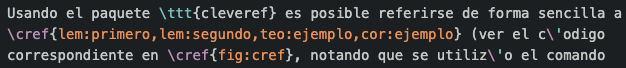
\includegraphics[width=0.8\textwidth]{recursos/capturas/cref}
  \caption{Ejemplo de uso de \ttt{\textbackslash{cref}}.}
  \label{fig:cref}
\end{figure}

Sin embargo, la gram\'atica del espa\~nol hace necesario introducir variantes en
algunos casos especiales, como cuando hacemos referencia ``al Teorema
\ref{teo:ejemplo}'' (n\'otese que se utiliz\'o ``al Teorema'' en lugar de ``el
Teorema''), o queremos decir que un resultado es una consecuencia ``del
Corolario \ref{cor:ejemplo}''.   En este caso, necesitamos agregar el nombre del
ambiente a mano, y usar el comando habitual \ttt{\textbackslash{ref}}.   El
autor del presente documento prefiere utilizar siempre may\'usculas cuando se
usa el nombre de un ambiente referido por n\'umero, e.g., ``\cref{teo:ejemplo}''
en lugar de ``el teorema \ref{teo:ejemplo}'', por lo que esta configuraci\'on se
ve reflejada en el archivo \ttt{tesis.tex}, cuando se utiliza el comando
\ttt{\textbackslash{crefname}} para definir los nombres de ambiente que debe de
usar \ttt{cleveref}.

Una alternativa para evitar algunos de los problemas descritos en el p\'arrafo
anterior es definir el nombre del ambiente sin utilizar el art\'iculo, e.g.,
``Teorema'' en lugar de ``el Teorema''.   Aunque esto permite un poco m\'as de
flexibilidad, cuando es necesario cambiar un ambiente con nombre masculino a uno
con nombre femenino, o viceversa (por ejemplo proposici\'on por lema), es
necesario realizar todos los cambios de los art\'iculos a mano.  Adicionalmente,
(y el motivo principal por el que se decidi\'o no usar esta variante) el uso del
paquete como el mostrado en el ejemplo de \cref{fig:cref} dejar\'ia de
funcionar, pues los art\'iculos ser\'ian omitidos, generando una construcci\'on
gramatical incorrecta.

Si no se desea usar el paquete \ttt{cleveref}, siempre puede omitirse y utilizar
\'unicamente el comando \ttt{\textbackslash{ref}} que est\'a incluido por
omisi\'on en \LaTeX.

Adem\'as de los ambientes, tambi\'en es posible etiquetar cap\'itulos o
secciones, y referirnos a la p\'agina donde aparece una etiqueta dada.   Por
ejemplo, podemos referirnos a \cref{sec:dibujos} en la \cpageref{sec:dibujos}, o
al Cap\'itulo \ref{cap:ejemplos}.   La referencia a las p\'aginas es \'util en
la versi\'on impresa del documento, aunque en la versi\'on digital parezca un
poco in\'util gracias a que cada referencia es una liga al objeto en cuesti\'on.



\section{Dibujos y colores}
\label{sec:dibujos}

Los dibujos pueden agregarse de al menos dos formas obvias.   La primera es
hacerlos dentro de \LaTeX con alg\'un paquete como
\href{https://github.com/pgf-tikz/pgf}{\ttt{tikz}}\index{tikz}.   La segunda es
generarlos con alg\'un recurso externo, e incluirlo con el comando
\ttt{\textbackslash{includegraphics}}.   Tambi\'en puede usarse una
combinaci\'on de ambos, generando un PDF con la imagen en un archivo externo de
\LaTeX, y agreg\'andolo con \ttt{\textbackslash{includegraphics}}; una ventaja
de esta tercera posibilidad es que el compilador realiza menos trabajo para
generar el documento.

En \cref{fig:grafica} podemos ver un ejemplo de un dibujo hecho con \ttt{tikz}.
Una ventaja de hacer los dibujos dentro de \LaTeX{} es que resulta f\'acil
agregar f\'ormulas o etiquetas con la misma tipograf\'ia que el resto del
documento.

\begin{figure}[ht!]
\centering
\begin{tikzpicture}
\node (0) [vertex,label=180:$v_1$] at (0,0){}; \node (1) [vertex,label=90:$v_2$]
at (1,0){};
\begin{scope}[xshift=2cm]
\node (2) [vertex,label=90:$v_3$]  at (270:1){}; \node (3)
[vertex,label=0:$v_4$]   at (0:1){}; \node (4) [vertex,label=90:$v_5$]  at
(90:1){};
\end{scope}

\draw [myloop,in=60,out=120,looseness=12]
      (0) to node[above]{$e_1$} (0);
\draw [myloop,in=240,out=300,looseness=12]
      (0) to node[below]{$e_2$} (0);
\draw [myloop,in=240,out=300,looseness=12]
      (2) to node[below]{$e_9$} (2);

\draw [edge]               (0) to node [above] {$e_3$} (1); \draw [edge]
(1) to node [below] {$e_4$} (2); \draw [edge]               (2) to node [below]
{$e_5$} (3); \draw [edge,bend right=20] (3) to node [above] {$e_6$} (4); \draw
[edge,bend left=20]  (3) to node [below] {$e_7$} (4); \draw [edge]
(4) to node [above] {$e_8$} (1);


% Componente derecha
\begin{scope}[xshift=6cm]
\node (5) [vertex,label=90:$v_6$]    at (0:1.5){}; \node (6)
[vertex,label=120:$v_7$]   at (120:1.5){}; \node (7) [vertex,label=240:$v_8$]
at (240:1.5){}; \node (8) [vertex,label=0:$v_9$]     at (3,1.2){}; \node (9)
[vertex,label=0:$v_{10}$]  at (3,-1.2){};

\draw [edge,bend right=10] (5) to node [above] {$e_{10}$} (6); \draw [edge,bend
left=10]  (5) to node [below] {$e_{11}$} (6); \draw [edge,bend right=10] (6) to
node [left]  {$e_{12}$} (7); \draw [edge,bend left=10]  (6) to node [right]
{$e_{13}$} (7); \draw [edge,bend right=10] (7) to node [below] {$e_{14}$} (5);
\draw [edge,bend left=10]  (7) to node [above] {$e_{15}$} (5); \draw [edge]
(5) to node [above] {$e_{16}$} (8); \draw [edge]               (5) to node
[below] {$e_{17}$} (9);
\end{scope}

\end{tikzpicture}
\caption{El diagrama de una gr\'afica con lazos y aristas m\'ultiples.}
\label{fig:grafica}
\end{figure}

Es f\'acil agregar colores a los dibujos.   Hay que tener presente que
\ttt{tikz} construye el dibujo por capas, y el c\'odigo se ejecuta de forma
secuencial, por lo que la \'ultima parte del c\'odigo es la \'ultima capa que se
dibujar\'a, y puede cubrir a otras, generando un resultado distinto al deseado.
Es posible definir colores nuevos mediante el comando
\ttt{\textbackslash{definecolor}}, en el caso de este documento, todos los
colores nuevos se definen en el archivo \ttt{tesis.tex}.   Las diferentes
opciones para el comando \ttt{\textbackslash{definecolor}} se encuentran
explicadas \href{https://en.wikibooks.org/wiki/LaTeX/Colors}{aqu\'i}.

Para agregar colores en el texto, o en las celdas de una tabla, u otros lugares,
se puede utilizar el paquete
\href{https://ctan.org/pkg/xcolor}{\ttt{xcolor}}\index{xcolor}.  Una forma
sencilla de usar color en el texto es con la construcci\'on
\begin{lstlisting}
{\color{nombre-del-color}texto con color}}
\end{lstlisting}
{\color{verdeAzulado}lo que permite generar texto de color.

Incluso es posible usar un color a lo largo de distintos p\'arrafos.}


\begin{figure}[ht!]
\begin{tikzpicture}
%%%%%%%%%%%%%%%%%%%%%%%%%%%%%%%%%%%%%%%%%%%%%%%%
%%%%%%%%%%         Empty Graph        %%%%%%%%%%
%%%%%%%%%%%%%%%%%%%%%%%%%%%%%%%%%%%%%%%%%%%%%%%%
\begin{scope}
% if label is needed -> label={(360/4)*\i}:$\i$
\foreach \i in {0,...,3} \node (\i) [vertex,fill=cyan] at ({(360/4)*\i}:1){};

\node (L) at (-1,1){$G_1$};
\end{scope}

%%%%%%%%%%%%%%%%%%%%%%%%%%%%%%%%%%%%%%%%%%%%%%%%
%%%%%%%%%%       Complete Graph       %%%%%%%%%%
%%%%%%%%%%%%%%%%%%%%%%%%%%%%%%%%%%%%%%%%%%%%%%%%
\begin{scope}[xshift=3.1cm,yshift=-0.3cm]
\node (4) [vertex,fill=verdeAzulado] at (0,0){}; \foreach \i in {0,1,2} \node
(\i) [vertex,fill=verdeAzulado] at ({90+(360/3)*\i}:1.2){};

\foreach \i in {0,1,2} \draw [edge] let \n1={int(mod(\i+1,3))} in (\i) to (\n1);
	\foreach \i in {0,1,2} \draw [edge] (\i) to (4);

\node (L) at (-1,1){$G_2$};
\end{scope}


%%%%%%%%%%%%%%%%%%%%%%%%%%%%%%%%%%%%%%%%%%%%%%%%
%%%%%%%%%%       Bipartite Graph      %%%%%%%%%%
%%%%%%%%%%%%%%%%%%%%%%%%%%%%%%%%%%%%%%%%%%%%%%%%
\begin{scope}[xshift=6.2cm,yshift=0cm]
\foreach \i in {0,2,4} \node (\i) [vertex,fill=red]  at ({(360/6)*\i}:1){};
	\foreach \i in {1,3,5} \node (\i) [vertex,fill=blue] at ({(360/6)*\i}:1){};

\foreach \i in {0,...,5} \draw [edge] let \n1={int(mod(\i+1,6))} in (\i) to
	(\n1);

\node (L) at (-1,1){$G_3$};
\end{scope}


%%%%%%%%%%%%%%%%%%%%%%%%%%%%%%%%%%%%%%%%%%%%%%%%
%%%%%%%%%%            Star            %%%%%%%%%%
%%%%%%%%%%%%%%%%%%%%%%%%%%%%%%%%%%%%%%%%%%%%%%%%
\begin{scope}[xshift=9.3cm]
\node (6) [vertex,fill=violet] at (0,0){}; \foreach \i in {0,...,4} \node (\i)
[vertex,fill=green] at ({90+(360/5)*\i}:1){};

\foreach \i in {0,...,4} \draw [edge] (\i) to (6);

\node (L) at (-1,1){$G_4$};
\end{scope}


%%%%%%%%%%%%%%%%%%%%%%%%%%%%%%%%%%%%%%%%%%%%%%%%
%%%%%%%%%%           Split            %%%%%%%%%%
%%%%%%%%%%%%%%%%%%%%%%%%%%%%%%%%%%%%%%%%%%%%%%%%
\begin{scope}[xshift=12.4cm]
\foreach \i in {0,2,4} \node (\i) [vertex,fill=black] at
	({30+(360/6)*\i}:0.7){}; \foreach \i in {1,3,5} \node (\i) [vertex] at
	({30+(360/6)*\i}:1.4){};

\foreach \i in {0,...,5} \draw [edge] let \n1={int(mod(\i+1,6))} in (\i) to
	(\n1); \foreach \i in {0,2,4} \draw [edge] let \n1={int(mod(\i+2,6))} in (\i)
	to (\n1);

\node (L) at (-1,1){$G_5$};
\end{scope}

\end{tikzpicture}
\caption{Ejemplos de gr\'aficas vac\'ia, completa, bipartita, bipartita completa
y escindible.}
\label{fig:fam1}
\end{figure}

Continuando con los dibujos, resulta bastante \'util usar ciclos \ttt{for}
dentro de \ttt{tikz} para realizar dibujos que tienen simetr\'ias.   Un ejemplo
de esto ocurre en \cref{fig:fam1}.   En \cref{fig:tikzFor}, se observa el
c\'odigo del ciclo azul y rojo que aparece en \cref{fig:fam1}.

\begin{figure}[ht!]
  \centering
  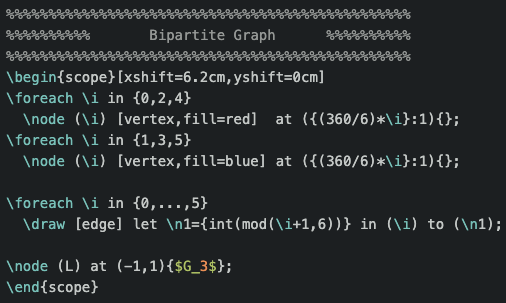
\includegraphics[width=0.8\textwidth]{recursos/capturas/tikzfor}
  \caption{Ejemplo de un ciclo \ttt{for} dentro de \ttt{tikz}.}
  \label{fig:tikzFor}
\end{figure}

Aunque en este caso los ejemplos se concentran en dibujar gr\'aficas, las
posibilidades de \ttt{tikz} son gigantescas.   Se recomienda al usuario revisar
el \href{https://mirror.las.iastate.edu/tex-archive/graphics/pgf/base/doc/%
pgfmanual.pdf}{manual de PGF y TikZ}.


\section{Algoritmos}

Para los algoritmos utilizamos el paquete \href{https://www.ctan.org/pkg/%
algorithm2e}{\ttt{algorithm2e}}\index{algorithm2e}.   En este caso simplemente
se presentar\'a un ejemplo de uso con un subconjunto limitado de las distintas
opciones que se pueden utilizar.   Se recomienda revisar la documentaci\'on del
paquete para conocer todas las posibilidades.

\begin{algorithm}[ht!]
\SetAlgorithmName{Algoritmo}{} \DontPrintSemicolon
  \SetKwData{False}{false}\SetKwData{True}{true}
  \SetKwFunction{New}{new}\SetKwFunction{End}{end}\SetKwFunction{Used}{used}
  \SetKwInOut{Input}{input}\SetKwInOut{Output}{output}

  \KwIn{Una gr\'afica conexa $G$ con un v\'ertice distingido $r$.}
  \KwOut{Funciones de parentesco $p$, nivel $\ell$ y tiempo de exploraci\'on
  $t$.} \BlankLine $Q \leftarrow []$; $i \leftarrow 0$\; $i \leftarrow i+1$\;
  colorear a $r$ de negro\; a\~nadir $r$ al final de $Q$\; $t(r) \leftarrow i$,
  $p(r) \leftarrow \varnothing$, $\ell (r) \leftarrow 0$\; {\While{$Q \ne []$}{
  elegir a la cabeza $x$ de $Q$\; \If{$x$ tiene un vecino $y$ sin colorear}{ $i
  \leftarrow i+1$\; colorear a $y$ de negro\; a\~nadir $y$ al final de $Q$\;
  $t(y) \leftarrow i$, $p(y) \leftarrow x$, $\ell(y) \leftarrow \ell(x) + 1$\;
  }\Else{ eliminar $x$ de $Q$\; } } } {\Return $(p,\ell,t)$}
  \caption{Breadth First Search}
  \label{alg:bfs}
\DecMargin{1em}
\end{algorithm}

\Cref{alg:bfs} muestra algunas opciones sencillas del paquete.   Quiz\'a la
observaci\'on m\'as importante para considerar respecto a \ttt{algorithm2e} es
que, por dise\~no, el paquete no divide los algoritmos para aparecer en m\'as de
una p\'agina.   Por lo tanto, un algoritmo largo usualmente se recorrer\'a a la
siguiente p\'agina (y posiblemente ocupar\'a una p\'agina completa).

\section{\'Indice alfab\'etico}
\label{sec:indice}

Es posible agregar palabras al \'indice\index{indice@\'indice} alfab\'etico
usando el comando \ttt{\textbackslash{index}}.   Un uso t\'ipico es el
siguiente; supongamos que se desea agregar la palabra ``gr\'afica'' al \'indice,
entonces es necesario escribir la palabra, seguida de la misma palabra dentro
del comando.
\begin{lstlisting}
gr\'afica\index{gr\'afica}
\end{lstlisting}

Cuando se introduce un concepto nuevo, es deseable resaltarlo de alguna forma en
el texto.   En los art\'iculos usualmente se utilizan \textit{cursivas} y en los
libros (o una tesis), generalmente se prefieren las \textbf{negritas}.   Por
este motivo, se agreg\'o al pre\'ambulo un comando para poner, al mismo tiempo,
una palabra en negritas y agregarla al \'indice; el comando es
\ttt{\textbackslash{indice}}.   Por ejemplo, dicho comando est\'a siendo
utilizado en la palabra \indice{concepto}, mismo que se puede verificar aparece
en el \'indice anal\'itico al final del documento. Tambi\'en es com\'un
encontrar una versi\'on especializada de un concepto, e.g., la definici\'on de
gr\'afica bipartita depende de la de gr\'afica.   En este sentido, es deseable
que ``gr\'afica bipartita'' aparezca como una entrada que depende de
``gr\'afica''.   Para lograr esto se utiliza el mismo comando
\ttt{\textbackslash{index}}, con la siguiente sintaxis.
\begin{lstlisting}
\index{concepto!subconcepto}
\end{lstlisting}

De manera an\'aloga al caso del comando \ttt{\textbackslash{indice}}, se cre\'o
un comando \ttt{\textbackslash{indiceSub}}, que toma dos argumentos.  El primero
es la entrada principal que aparecer\'a en el \'indice (e.g., gr\'afica), y la
segunda es la versi\'on especializada que depende de la primera (e.g.,
bipartita).   Para brindar libertad en la forma de redactar las definiciones,
\ttt{\textbackslash{indiceSub}} s\'olo imprime en el documento el segundo
argumento.   Por ejemplo, en \indiceSub{concepto}{subconcepto} se utiliz\'o
\ttt{\textbackslash{indiceSub}} con los argumentos \ttt{concepto} y
\ttt{subconcepto} (puede verificarse el funcionamiento en el \'indice).

Dependiendo del editor que se est\'e utilizando para trabajar con \LaTeX, es
posible que el \'indice no se actualice autom\'aticamente.   De ser el caso,
basta con ejecutar el siguiente comando en el directorio del proyecto donde se
encuentre el archivo \ttt{tesis.idx} (\'este \'ultimo se genera
autom\'aticamente al compilar \ttt{tesis.tex}).
\lstset{language=bash}
\begin{lstlisting}
makeindex tesis.idx
\end{lstlisting}

El comando anterior generar\'a el archivo \ttt{tesis.ind}, mismo que contiene la
informaci\'on necesaria para incluir el \'indice en el PDF final.

Los conceptos aparecen en orden alfab\'etico en el \'indice, sin embargo, el uso
de caracteres especiales (como letras acentuadas) afecta el orden habitual. Para
corregir problemas derivados del uso de caracteres especiales, se refiere al
lector al siguiente \href{https://en.wikibooks.org/wiki/LaTeX/%
Indexing#Using_special_characters}{art\'iculo sobre indexaci\'on}.
\end{comment}